% Some commands used in this file
\newcommand{\package}{\emph}

\chapter{Introduction}

In the study of astrophysical entities, accretion shocks are a fairly commonly encountered physical phenomena. In particular, standing accretion shocks (SAS) are part of the theory behind core-collapse supernovae, with an instability (SASI) described by Blondin et al.~\cite{Blondin2003} being proposed as a possible mechanism for driving the explosive evolution of these phsyical systems. This instability occurs because of the spherical nature of the system, with the effects of perturbations to the symmetry of the shock being trapped in the interior subsonic region and producing feedback loops which further perturb the shock front.

To gain a better understanding of the underlying mechanisms of this instability, Foglizzo~\cite{Foglizzo2009} and Sato et al.~\cite{Sato2009} (hereafter referred to together as FS) proposed and studied a simple toy problem, the details of which are presented in Section \ref{sec:toyProblem}. Using this simple set-up they showed evidence for a coupled advective-acoustic cycle between the stationary shock front and an interior decelerating potential step that is intended to model the effects of matter settling onto the surface of the accreting object.

For this thesis, well-balanced methods for simulating steady states in the presence of external potential fieds, as developed by K\"appeli and Mishra~\cite{Kappeli2014} (hereafter referred to as KM), were applied to the aforementioned toy problem as well as 2D simulations of the SASI scenario using circular and spherical geometries. The mathematical theory of fluid flow and associated steady states is briefly outlined in Section~\ref{sec:euler} while an overview of the numerical method and well-balanced scheme used for this thesis is given in Section~\ref{sec:numerics}.


\section{Euler Equations}
\label{sec:euler}

The time evolution of the dynamics of fluids can be described by systems of balance laws. For inviscid fluids, this system is given by the well-known Euler equations with source terms, which mathematically represent the physical conservation of mass, momentum, and energy. They are given here following the notation of KM as
\begin{align} \label{eq:eulerFull}
\frac{\partial{\rho}}{\partial{t}} &+ \nabla \cdot (\rho \mathbf{v}) = 0,\\
\frac{\partial{\rho \mathbf{v}}}{\partial{t}} &+ \nabla \cdot (\mathbf{v} \rho \mathbf{v}) + \nabla p = -\rho \nabla \phi,\\
\frac{\partial{E}}{\partial{t}} &+ \nabla \cdot \left[(E+p)\mathbf{v}\right] = -\rho \mathbf{v} \cdot \nabla \phi,
\end{align}
where $\rho$ is the mass density, and $\mathbf{v}$ is the local velocity vector. $E$ is the total energy sum of the internal and kinetic energies given as $$E=\rho e + \frac{\rho v^2}{2}.$$  An equation of state $p=p(\rho,e)$ must be selected for a given problem to complete the relations between these primitive quanitites. The quantitiy $\phi$ on the right-hand side of the latter two equations represents an external potential field (e.g.\ gravity) which acts upon the fluid. For our purposes, this potential is assumed to be known, either as a given value, through pre-computation, or by solving for it independently of the other fluid quantities at each time step.

The Euler system of equations can be rewritten in the condensed form of a general balance law as
\begin{equation} \label{eq:euler}
\mathbf{U}_t+\nabla\cdot(\mathbf{F}(\mathbf{U}))=\mathbf{S}(\mathbf{U}),
\end{equation}
where $\mathbf{U}$ is a vector of the conserved quantities, and $\mathbf{F}$ and $\mathbf{S}$ represent the fluxes and sources of these quanitites in the system.

\subsection{Steady States}

For fluid flows in the presence of an external potential field, non-trivial steady states (also called stationary solutions) can arise. Highly accurate simulations of these stationary solutions are of interest as they allow for accurate reproduction and analysis of subsequent perturbations to the system, which can be quite small and therefore overwhelmed by the truncation error of a less well-resolved scheme.

It can be seen that for a steady state solution the time derivative term is exactly zero and the conservation law~(\ref{eq:euler}) reduces to a balance between the fluxes and sources as
\begin{equation}
\nabla\cdot(\mathbf{F}(\mathbf{U}))=\mathbf{S}(\mathbf{U}).
\end{equation}


\section{Toy Problem}
\label{sec:toyProblem}

As previously mentioned, for an initial test of our well-balanced  to the SASI, the simple toy model of FS was chosen. The salient details from those papers  \cite{Foglizzo2009,Sato2009} are reproduced here. Following the notation of FS, we will denote quantities in the supersonic region before the shock with a subscript ``1'', in the interior region between the shock and potential step with ``in'', and in the outflow region past the step with ``out''.

A schematic view of the problem domain can be seen in Fig.~\ref{fig:Sato1}, showing how the overall scenario is split into two sub-problems for simulation. The entire test case consists of an supersonic inflow deccelerated at a stationary shock front, followed shortly after by a potential step which further slows the now subsonic flow. This provides a very simplistic analogue to study the mechanisms at play during the inflow, decceleration, and accredtion of matter in a collapsing star before supernova.

\begin {figure}
\centering
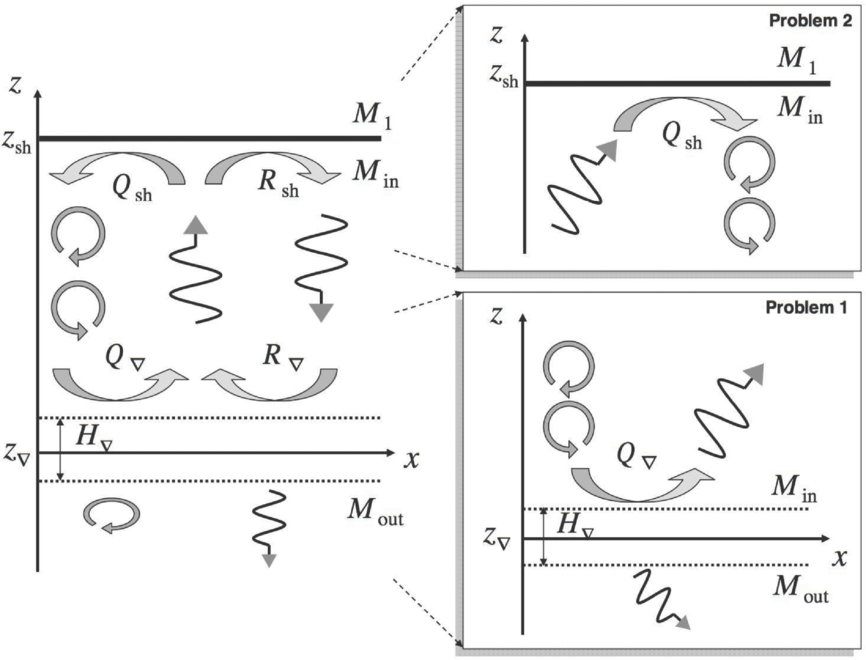
\includegraphics[width=10cm]{figures/Sato1}
\caption {A short caption.}
\label{fig:Sato1}
\end{figure}

For ease of simulation, the potential step and stationary shock are computed separately as sub-problems 1 and 2 respectively. This separation greatly simplifies the introduciton of specific advective and acoustic pertubations to locations in the domain, making it much easier to see the interactions of these disturbances at the boundaries of the various flow regions.


\subsection{Sub-Problem 1}

Description of potential step

\subsection{Sub-Problem 2}

Description of the standing shock


\section{Numerics}
\label{sec:numerics}

It has been well-studied that the non-linear nature of the Euler equations~(\ref{eq:eulerFull}) can lead to very complicated flow features and shocks, even from initially smooth conditions. As such, numerical solutions to these systems can only be found in a weak sense, and require some other thermodynamic information, e.g. regarding the entropy or temperature to fix a unique solution. Many methods have therefore been developed to resolve such flows in a stable and consistent manner, with one of the most popular being the class of finite volume methods (FVM).

A typical FVM discretizes the domain into small cells (or volumes) and then evolves the cell averages of the conserved quantities by computing their fluxes at all of the faces between adjacent volumes. As the values in adjacent cells differ in general, a Riemann problem will appear at each cell interface which can then be solved to obtain the fluxes. Exact solutions are possible and are the basis of the so-called Godunov schemes~\cite{Godunov1959}, but usually the computational effort is saved by using an approximate solution, such as from a Roe~\cite{Roe1981}, Rusanov~\cite{Rusanov1961}, or HLLC~\cite{Toro1994} solver, as the rest of the method is itself only approximate due to truncation error.

\subsection{Well-Balanced Reconstruction}
\label{subsec:wellBalanced}

Up to second-order accuracy the cell average value is equivalent to the value at the cell centre, and so some method of approximating the values at the cell interfaces must be selected. As such, a FVM also requires one to specifiy a reconstruction scheme to extend these values stored at the cell centres to the cell edges to obtain the Riemann problem at that interface. A piecewise constant reconstruction where the cell average value is simply used at the interface is the simplest such scheme, but gives only first-order accuracy.

Second-order accuracy can be achieved by computing the gradient at each cell centre and using that to linearly extrapolate to the cell edges. However, this method generally gives rise to spurious oscillations in the resulting solutions, particularly near sharp flow features such as shock fronts. To counter this, most such schemes limit the gradient in areas of rapid change, reducing the local order of accuracy towards first-order. Such schemes are referred to as total variation diminishing (TVD) and various slope limiter functions such as those by Barth and Jespersen~\cite{Barth1989}, Venkatakrishnan~\cite{Venkatakrishnan1993,Venkatakrishnan1995}, or Michalak and Gooch~\cite{Michalak2008}.

Therefore, it is desirable to use a scheme for which these terms are exactly balanced for an equilibrium stationary solution. Such a method has been developed by KM, termed a well-balanced scheme, and the salient results of their derivations are reproduced here.

